% =====================================================================
% cosmos3edge_teaser.tex  --  camera-ready TikZ teaser figure
% Cosmos3-Edge (4B) for Connectomics Segmentation
% ---------------------------------------------------------------------
% Standalone vector figure for SIGGRAPH / IEEE TVCG / IEEE TMI / MedIA.
% Compile:  pdflatex cosmos3edge_teaser.tex   (-> tight-cropped PDF)
% Drop into a paper:  \input{cosmos3edge_teaser_body.tex} inside a figure*,
% or \includegraphics the compiled PDF.
% =====================================================================
\documentclass[tikz,border=4pt]{standalone}
\usepackage{fontspec}            % comment out + use pdflatex if no system fonts
\usepackage{tikz}
\usetikzlibrary{arrows.meta,positioning,backgrounds,fit,calc}

% ---- restrained, colour-blind-safe palette -------------------------------
\definecolor{ink}{HTML}{1B2430}
\definecolor{inF}{HTML}{EEF1F5}\definecolor{inE}{HTML}{3B4A5A}
\definecolor{sslF}{HTML}{DCEEE4}\definecolor{sslE}{HTML}{2E7D55}
\definecolor{sftF}{HTML}{DBE6F6}\definecolor{sftE}{HTML}{2C5C9E}
\definecolor{vaeF}{HTML}{D6EDEA}\definecolor{vaeE}{HTML}{1F7A72}
\definecolor{ditF}{HTML}{E8E1F4}\definecolor{ditE}{HTML}{5B3E9B}
\definecolor{headF}{HTML}{FBEED9}\definecolor{headE}{HTML}{B5791F}
\definecolor{poolF}{HTML}{EAE6F3}\definecolor{poolE}{HTML}{6A52A3}
\definecolor{lossF}{HTML}{F3E7EF}\definecolor{lossE}{HTML}{9C3F7A}
\definecolor{mwsF}{HTML}{FAE3D4}\definecolor{mwsE}{HTML}{C2541B}

\begin{document}
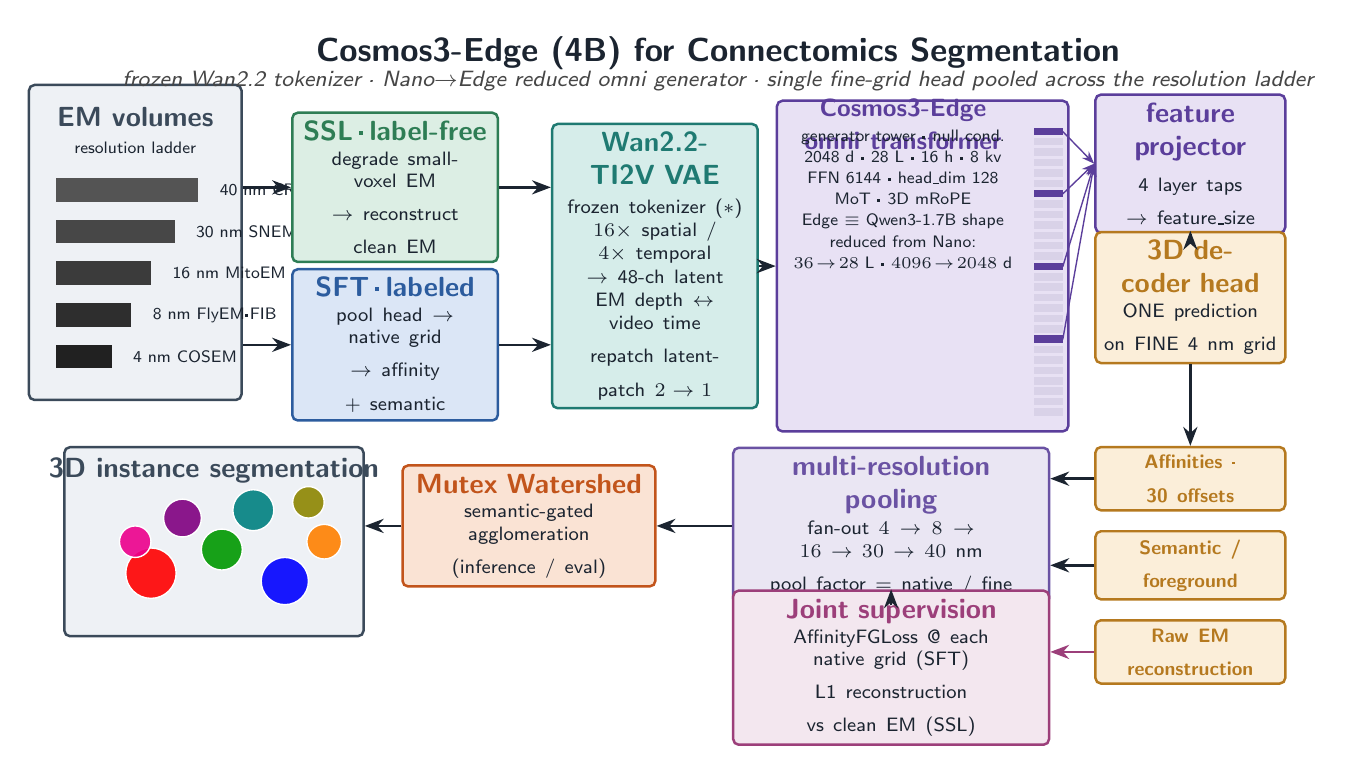
\begin{tikzpicture}[
  x=1mm,y=1mm,
  font=\sffamily,
  panel/.style={rounded corners=2pt,draw,line width=0.9pt,align=center,
                inner sep=3pt,text=ink},
  ttl/.style={font=\sffamily\bfseries},
  sub/.style={font=\sffamily\fontsize{6.4}{7.6}\selectfont,text=ink},
  flow/.style={-{Stealth[length=2.4mm]},line width=0.9pt,ink},
  tap/.style={-{Stealth[length=1.6mm]},line width=0.5pt,ditE},
]

% ---------------- TOP ROW : backbone (left -> right) ----------------------
\node[panel,fill=inF,draw=inE,minimum width=27mm,minimum height=40mm] (in)
  at (16,72) {};
\node[ttl,text=inE] at (16,88) {EM volumes};
\node[sub] at (16,84) {resolution ladder};
% ladder bars
\foreach \i/\nm/\ds/\bw/\gy in {
   0/4 nm/COSEM/7/0.74, 1/8 nm/FlyEM·FIB/9.5/0.64, 2/16 nm/MitoEM/12/0.54,
   3/30 nm/SNEMI/15/0.44, 4/40 nm/CREMI·MICrONS/18/0.34}{
   \fill[gray!\fpeval{round((1-\gy)*100)}!black] (6,\fpeval{56+\i*5.3}) rectangle (\fpeval{6+\bw},\fpeval{59+\i*5.3});
   \node[sub,anchor=west] at (\fpeval{6+\bw+1.5},\fpeval{57.5+\i*5.3}) {\nm\ \ds};
}

\node[panel,fill=sslF,draw=sslE,text width=24mm,minimum height=15mm] (ssl) at (49,79)
  {\textbf{\textcolor{sslE}{SSL\,·\,label-free}}\\[1pt]\small\sffamily\fontsize{6.6}{8}\selectfont degrade small-voxel EM\\$\rightarrow$ reconstruct clean EM};
\node[panel,fill=sftF,draw=sftE,text width=24mm,minimum height=15mm] (sft) at (49,59)
  {\textbf{\textcolor{sftE}{SFT\,·\,labeled}}\\[1pt]\small\sffamily\fontsize{6.6}{8}\selectfont pool head $\rightarrow$ native grid\\$\rightarrow$ affinity + semantic};

\node[panel,fill=vaeF,draw=vaeE,text width=24mm,minimum height=26mm] (vae) at (82,69)
  {\textbf{\textcolor{vaeE}{Wan2.2-TI2V VAE}}\\[2pt]\small\sffamily\fontsize{6.6}{8.4}\selectfont frozen tokenizer ($\ast$)\\$16\times$ spatial / $4\times$ temporal\\$\rightarrow$ 48-ch latent\\EM depth $\leftrightarrow$ video time\\repatch latent-patch $2\!\to\!1$};

\node[panel,fill=ditF,draw=ditE,minimum width=37mm,minimum height=42mm] (dit) at (116,69) {};
\node[ttl,text=ditE,text width=29mm,align=center] at (113.5,87) {\fontsize{8.6}{10}\selectfont Cosmos3-Edge omni transformer};
\node[sub,align=center] at (113.5,77.5)
  {generator tower · null cond.\\ 2048 d · 28 L · 16 h · 8 kv\\ FFN 6144 · head\_dim 128\\ MoT · 3D mRoPE\\ Edge $\equiv$ Qwen3-1.7B shape\\ reduced from Nano:\\ $36\!\to\!28$ L · $4096\!\to\!2048$ d};
% layer-stack strip + taps
\foreach \i in {0,...,27}{
  \pgfmathtruncatemacro{\istap}{(\i==7)||(\i==14)||(\i==21)||(\i==27)}
  \ifnum\istap=1 \fill[ditE] (130.2,\fpeval{50+\i*1.32}) rectangle (133.8,\fpeval{50.95+\i*1.32});
  \else \fill[ditF!40!ditE!35] (130.2,\fpeval{50+\i*1.32}) rectangle (133.8,\fpeval{50.95+\i*1.32}); \fi
}

\node[panel,fill=ditF,draw=ditE,text width=22mm,minimum height=11mm] (proj) at (150,82)
  {\textbf{\textcolor{ditE}{feature projector}}\\[1pt]\small\sffamily\fontsize{6.6}{8}\selectfont 4 layer taps $\rightarrow$ feature\_size};
\node[panel,fill=headF,draw=headE,text width=22mm,minimum height=13mm] (head) at (150,65)
  {\textbf{\textcolor{headE}{3D decoder head}}\\[1pt]\small\sffamily\fontsize{6.6}{8}\selectfont ONE prediction\\on FINE 4 nm grid};

% ---------------- BOTTOM ROW : supervision & inference (right -> left) -----
\node[panel,fill=headF,draw=headE,text width=22mm,minimum height=8mm] (aff) at (150,42)
  {\small\sffamily\fontsize{7}{8.4}\selectfont\textbf{\textcolor{headE}{Affinities · 30 offsets}}};
\node[panel,fill=headF,draw=headE,text width=22mm,minimum height=8mm] (sem) at (150,31)
  {\small\sffamily\fontsize{7}{8.4}\selectfont\textbf{\textcolor{headE}{Semantic / foreground}}};
\node[panel,fill=headF,draw=headE,text width=22mm,minimum height=8mm] (raw) at (150,20)
  {\small\sffamily\fontsize{7}{8.4}\selectfont\textbf{\textcolor{headE}{Raw EM reconstruction}}};

\node[panel,fill=poolF,draw=poolE,text width=38mm,minimum height=14mm] (pool) at (112,36)
  {\textbf{\textcolor{poolE}{multi-resolution pooling}}\\[1pt]\small\sffamily\fontsize{6.8}{8.4}\selectfont fan-out $4\!\to\!8\!\to\!16\!\to\!30\!\to\!40$ nm\\ pool factor $=$ native / fine};
\node[panel,fill=lossF,draw=lossE,text width=38mm,minimum height=12mm] (loss) at (112,18)
  {\textbf{\textcolor{lossE}{Joint supervision}}\\[1pt]\small\sffamily\fontsize{6.6}{8}\selectfont AffinityFGLoss @ each native grid (SFT)\\ L1 reconstruction vs clean EM (SSL)};
\node[panel,fill=mwsF,draw=mwsE,text width=30mm,minimum height=14mm] (mws) at (66,36)
  {\textbf{\textcolor{mwsE}{Mutex Watershed}}\\[1pt]\small\sffamily\fontsize{6.6}{8}\selectfont semantic-gated agglomeration\\(inference / eval)};
\node[panel,fill=inF,draw=inE,minimum width=38mm,minimum height=24mm] (seg) at (26,34) {};
\node[ttl,text=inE] at (26,43) {3D instance segmentation};
\foreach \cx/\cy/\r/\col in {18/30/3.2/red, 27/33/2.6/green!60!black, 35/29/3/blue,
   40/34/2.2/orange, 22/37/2.4/violet, 31/38/2.6/teal, 38/39/2/olive, 16/34/2/magenta}{
   \fill[\col,opacity=0.9] (\cx,\cy) circle (\r); \draw[white,line width=0.5pt] (\cx,\cy) circle (\r);
}

% ---------------- arrows --------------------------------------------------
\draw[flow] (in.east|-ssl) -- (ssl.west);
\draw[flow] (in.east|-sft) -- (sft.west);
\draw[flow] (ssl.east) -- (vae.west|-ssl);
\draw[flow] (sft.east) -- (vae.west|-sft);
\draw[flow] (vae.east) -- (dit.west);
\foreach \ty in {7,14,21,27}{
  \draw[tap] (133.8,\fpeval{50.45+\ty*1.32}) -- (proj.west);
}
\draw[flow] (proj.south) -- (head.north);
\draw[flow] (head.south) -- ++(0,-3) -| (aff.north);   % head -> outputs
\draw[flow] (aff.west) -- (pool.east|-aff);
\draw[flow] (sem.west) -- (pool.east|-sem);
\draw[flow] (pool.south) -- (loss.north);
\draw[flow,lossE] (raw.west) -- (loss.east|-raw);
\draw[flow] (pool.west) -- (mws.east);
\draw[flow] (mws.west) -- (seg.east|-mws);

% ---------------- title ---------------------------------------------------
\node[ttl,text=ink,font=\sffamily\bfseries\fontsize{13}{15}\selectfont] at (90,96)
  {Cosmos3-Edge (4B) for Connectomics Segmentation};
\node[font=\sffamily\itshape\fontsize{8}{10}\selectfont,text=gray!55!black] at (90,92.5)
  {frozen Wan2.2 tokenizer\ ·\ Nano$\to$Edge reduced omni generator\ ·\ single fine-grid head pooled across the resolution ladder};
\end{tikzpicture}
\end{document}
